

\begin{frame}{web3: history}
\begin{block}{}
web 1.0
\end{block}
\begin{block}{}
web 2.0
\end{block}
\begin{block}{}
web3
\end{block}
\end{frame}


% \subsection{A (simplified) history of WWW Incentivisation}
% \subsubsection{Web 1.0}
\wholeslide{\Large{Incentive structure of Web 1.0}}
\begin{frame}{Incentive structure of Web 1.0}
  Back in the day...\\
  \begin{enumerate}
    \item<2-> Start up a webserver (or rent one)
    \item<3-> Upload some content (FTP)
  \end{enumerate}
  \begin{center}
    \begin{tabular}{ccc}
      \multicolumn{1}{l}{\uncover<4->{\textbf{Content is unpopular}}}	  & \multicolumn{2}{l}{\uncover<6->{\textbf{Content becomes popular}}}\\
      \multicolumn{1}{l}{\uncover<5->{$\bullet$ Pay running costs}}	  & \multicolumn{2}{l}{\uncover<7->{$\bullet$ Bandwidth costs skyrocket}}\\
      \multirow{2}{*}{\uncover<5->{
\includegraphics[scale=0.2]{smallcoinpile.png}}} & \multicolumn{2}{l}{\uncover<8->{$\bullet$ Server crashes and goes offline.}}\\
      & \uncover<7->{$\qquad$
\includegraphics[scale=0.2]{bigcoinpile.png}} & \uncover<8->{
\includegraphics[scale=0.2]{servercrash.jpg}}
    \end{tabular}
  \end{center}
 \begin{flushright}
  \uncover<9>{...but at least you owned your content.}
  \end{flushright}
\end{frame}

% \subsubsection{Web 2.0}
\wholeslide{\Large{Incentive structure of Web 2.0}}
\begin{frame}{Web 2.0}
 Today\alt<1>{...}{ we just upload our content to ``the cloud".}\\[5pt]
 \uncover<3->{The cloud is:}\\
 \begin{itemize}
  \item<3-> Cheap \uncover<4->{or even \alt<5->{``free"}{free}}
  \item<6-> Scalable
  \item<7-> Reliable
 \end{itemize}
 \uncover<8->{\Large{\alert{But...}}\\}
 \begin{itemize}
  \item<9-> Content is \alert<9>{owned by the service providers}.
  \item<10-> All users are \alert<10>{tracked and spied on}; providers profit off the data.
  \item<11-> Centralised control: \alert<11>{surveillance and censorship}.
 \end{itemize}
\pause
\end{frame}


% \subsubsection{Peer-to-peer (p2p)}
\blockslide{}{\Large{What about p2p?}}
\begin{frame}{Properties of the bittorrent network}
 \only<1>{Let's talk about }Bittorrent\\
 \uncover<2->{\textbf{Pros:}}
 \begin{itemize}
  \item<2-> Content is distributed among peers.
  \item<3-> Distribution scales automatically.
  \item<4-> Hashing ensures data integrity.
  \item<5-> No central point of failure (no servers).
 \end{itemize}
 \uncover<6->{\textbf{Cons:}}
 \begin{itemize}
  \item<6-> Downloads start slowly (high latency).
  \item<7-> No incentive to provide content: ``seeding".
 \end{itemize}
\end{frame}

% \subsubsection{Introduction}
\begin{frame}{Swarm Incentive System}
\begin{columns}[t]
  \column{.5\textwidth}
    \begin{block}<2->{Bandwidth}
     \uncover<3->{$\bullet$ Account for all bandwidth used (p2p).\\}
     \uncover<4->{$\bullet$ Compensate nodes based on provided bandwidth.}
    \end{block}
  \column{.5\textwidth}
    \begin{block}<2->{Storage}
      \uncover<5->{$\bullet$ Allow for long term storage of data.}\\
      \uncover<6->{$\bullet$ Provide proper compensation for nodes storing the data.}
    \end{block}
\end{columns}
\end{frame}


\begin{frame}{web3: promises}
\begin{block}{}
scalability
\end{block}
\begin{block}{}
  security
\end{block}
\begin{block}{}
sustainability
\end{block}
\end{frame}

\begin{frame}[plain,c]
\begin{center}
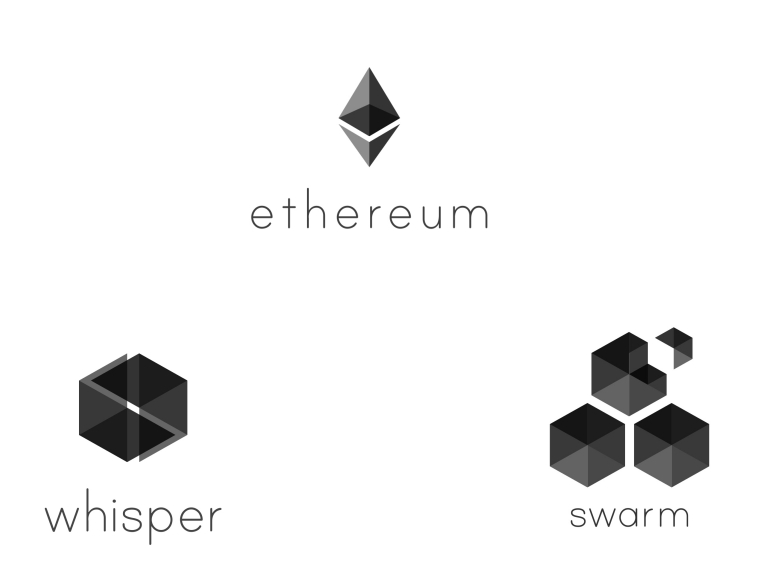
\includegraphics[width=0.8\textwidth]{ecosystem0.jpg}
\end{center}
\end{frame}


\begin{frame}{swarm}
\begin{block}{}
storage for web3: archival and retrieval monetized
\end{block}
\begin{block}{}
serving web applications with routed messaging
\end{block}
\begin{block}{}
silly world of acronyms, riddles and mnemonics
\end{block}
\end{frame}



% \begin{frame}
%  \tableofcontents[subsectionstyle=shaded/shaded,subsubsectionstyle=hide/hide]
% \end{frame}


%
% \begin{frame}
%  \tableofcontents[subsectionstyle=shaded/shaded,subsubsectionstyle=hide/hide]
% \end{frame}
